\chapter*{Introduction}
\label{cap:introduction}
\addcontentsline{toc}{chapter}{Introduction}

\chapterquote{Everything sinks into the fog of oblivion but when the fog clears, oblivion is full of memory}{Mario Benedetti}

\section{Motivation}

Our existence is essentially made up of experiences, unique and personal moments that mark the journey in each person's life. Our identity is formed with the set of events that we experience along the way and to preserve them, the brain stores them in the form of memories throughout our entire life.   From our first memory, which is normally between 2 and 4 years old, because the formation of new neurons prevents the hippocampus from storing memories until that age, a phenomenon known as infantile amnesia (Freud, 1895). Until the last one, which may be distorted or completely erased due to the deterioration of our brain and the inability of our neurons to make the possible connections for it. The latter case includes a degenerative disease commonly known as Alzheimer's, which currently affects more than 55 million people worldwide. However, it is not only these people who suffer from it, but everyone close to them as well. \\

\section{What is Alzheimer's?}

Alzheimer's is a disease that slowly destroys memory and, in addition, also deteriorates thoughts and behavior, until little by little the most basic functions are affected. Alzheimer's is the leading cause of dementia \citep{NationalInstitute2023}.\\

The brain sends chemical stimuli through neurons creating brain connections, and through billions of these connections, our memories, feelings, thoughts and locomotor abilities are obtained. Although the reason that causes this disease in the brain is still not known with certainty, it has been investigated that there are two proteins in the brain that become toxic over time, tau and beta-amyloid, which accumulate until they obstruct the connection between the neurons and cause them to die, as can be seen in \ref{fig:tau}.   With the destruction of neurons, the brain shrinks and with it also severely, the hippocampus, which is a fundamental key part of our brain when it comes to forming new memories and for learning, which causes our memory, our ability to make decisions and speech, fail. To help combat this disease there are pharmacological and non-pharmacological methods. In this project we will focus on the second group, more specifically, on reminiscence therapy. \\

\begin{figure}[h]
	\centering
	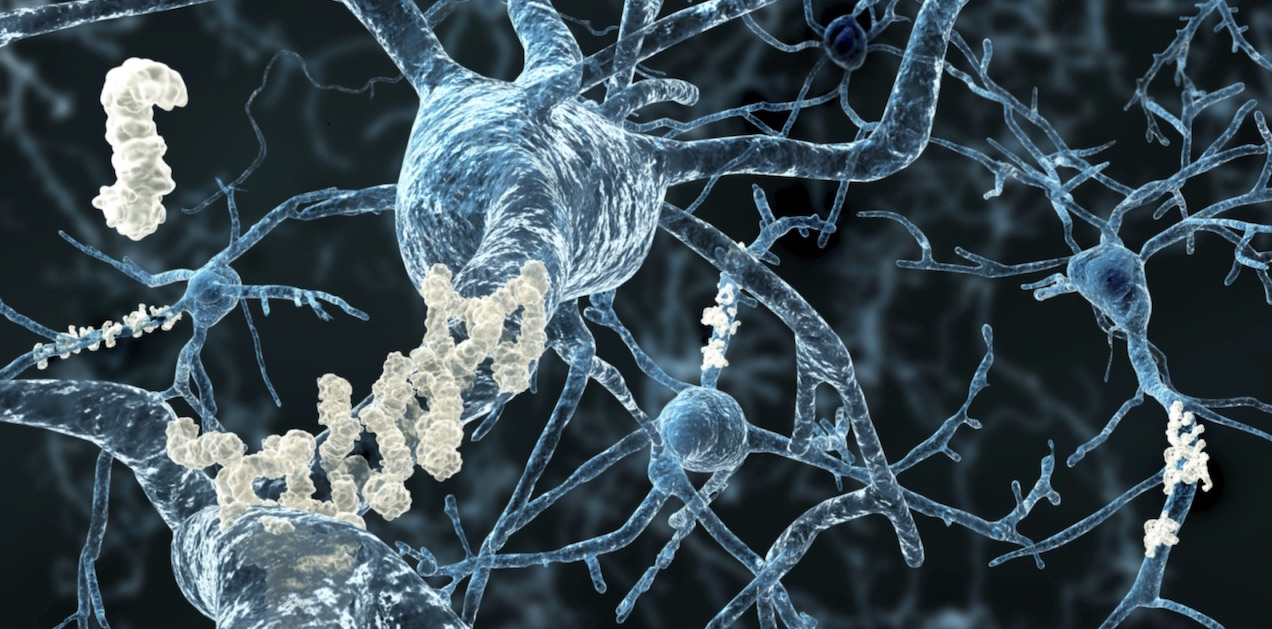
\includegraphics[width = 1 \textwidth]{Imagenes/Vectorial/proteina-tau.jpg}
	\caption{Clogging of neurons by vitamin tau \citep{tau}}
	\label{fig:tau}
\end{figure}


\section{Reminiscence therapy}

Fortunately, there are therapies that help improve the quality of life of people who suffer from this disease. Among them cognitive stimulation, reality orientation, therapeutic exercise, music therapy, and multisensory stimulation, among others \citep{SAS2020}.\\

Our project is linked to reminiscence therapy, which is a process that helps the person evoke emotional moments and experiences and integrate them into the present, which can improve self-esteem and quality of life \citep{gonzalez2015terapia}.\\

Specifically, the technique consists of showing the person a visual, musical or even olfactory tool or material, linked to their own experience or historical facts. In this way, a review of the person's life will be promoted, so that a connection is achieved with their experiences, in order to reconstruct a life book and reinforce their identity as a person.   This therapy can be classified as a type of daydreaming that takes them to their past, allowing them to enter a state of concentration in order to strengthen their general memory, which strengthens the brain and develops their social abilities, stimulates memories. through sensory organs and activates their sense of identity.\\



Some of the benefits of life book creation and reminiscence occupational therapy, among many others, are:\\
\begin{itemize}
	\item \underline{Emotional well-being}: It allows people to remember positive and significant experiences in their lives, which can generate satisfactory feelings of joy and happiness.\\
	\ item \ underline {Self-knowledge}: When a person reviews and reflects on past events and personal achievements, he can gain an understanding of himself. Through the interaction of his memories, aided by the guidance of caregivers and therapists, he is able to evoke aspects of his values, strengths and weaknesses that would not otherwise be accessible.
	\item \underline{Personal meaning and purpose}: By recalling significant scenes, people can find emotional guidance that allows them to give meaning and direction to their lives, especially in times of confusion or disorientation.
	\item \underline{Stress reduction}: By focusing on positive memories, people experience a sense of calm, tranquility and emotional well-being, and find a space to escape the stress and tensions of the present.
	\item \underline{Promote social relationships}: Sharing memories and experiences with other people can strengthen social ties and foster a greater connection with caregivers, family and friends, which is highly satisfactory for the patient.
	\item \underline{Increase language and person development}: By recounting past experiences, people improve their ability to communicate effectively as well as their verbal expression, which drives significant emotional and intellectual personal growth.
	\item \underline{Prevent disability}: Strengthening language skills and keeping the mind active can help preserve cognitive function over time. 
	\end{itemize}
	
	
	
	In summary, it is recommended to carry out occupational therapy activities because they improve the quality of life of patients, because personal and life satisfaction is achieved, attention, memory and language are stimulated, moments are relived. meaningful and emotional and socialization is encouraged. All of this leads to delaying possible cognitive problems \citep{SAS2020}.\\
	
	\section{About the project}
	
	Given these benefits, the initiative to carry out this project was born, as it is a visual support tool for the narration of life books. A life book is a compilation of the most important and characteristic events of a person throughout their life, adding visual support and usually being organized by stages. The characteristic of a life book is to give a context to the incorporated images so that what has been experienced can be understood in a timeline, which helps to enhance the person's memory and their sense of identity \citep{life book }. 
	
	To create it, we will use artificial intelligence techniques that convert text inputs to images and in this way, we will be able to transform memories narrated by the patient and convert them into images that correspond to the memory described. The interesting thing is to be able to give the possibility of making these images more personal so that a series of images of one's own, of family members or of important events in the patient's life can be added, to train the generative artificial intelligence model in charge of carrying out the process. of creating the images, and that the final result is unique, special and of great help to the person who suffers from this disease. 
	
	The work was born based on the CANTOR project (Automatic Composition of Personal Narratives to support Occupational Therapy based on Reminiscence, National Research Plan), an initiative proposed by researchers from a group of Spanish universities, including the Complutense University of Madrid.
	
	The main motivation for the creation of this project is to provide the possibility for patients with dementia caused by Alzheimer's to build a book made up of their happiest memories, giving them the opportunity to remember them. It has been shown that when patients talk about certain times in their lives and moments experienced in the past, a positive impact is generated on them, increasing their confidence and identity \citep{UCMcantor}.\\
	
The CANTOR project is designed to be carried out in two stages: 
\begin{itemize}
	\item The first would be the technical part in which a tool is developed to automate the construction of the life book using artificial intelligence. 
	\item The second stage consists of taking the tool to the therapists and people who assist those affected to check its functionality and effectiveness. 
\end{itemize}

We will focus on addressing the first stage of the project, making sure to implement a tool capable of generating images through an artificial intelligence technique specialized in this, in a way that ensures the maximum possible quality in the results and ensuring a practically total resemblance to reality. That is, our objective is to create a tool that is capable of helping in the process of reminiscence therapy for the creation of a life book of a certain patient, so that visual representations can be created from descriptions that the person contribution of certain memories. The usefulness and purpose of creating images from text using a trained artificial intelligence technique is to obtain personal images to remember moments in your life that are not immortalized in a photograph or that you do not have access to. \\

For it to be possible to generate personal images through artificial intelligence methods, it is necessary for family members to provide a sufficiently large number of photographs of the patient at different stages of their life (minimum 10 of each), or of people, places, animals or objects that may be meaningful to him or her. The purpose is to teach the artificial intelligence model designed to generate images to identify the desired element. And thus, obtaining as a result a personalized image of the person to serve as support in reminiscence therapy, to be included in the person's life book and to generate a positive impact on their mental well-being \\.


\section{Goals}

For the correct completion of the project and in order to obtain the best possible results, we have established some objectives to guide us during the preparation of the work and keep in mind at all times the path we will take to carry it out. 

\begin{itemize}
	\item Study the different artificial intelligence techniques in order to choose the most appropriate one for generating images. 
	\item Analyze the necessary characteristics of the input data set for effective training of the artificial intelligence model. 
	\item Use generative artificial intelligence to create personal images that help patients evoke emotional moments and experiences and integrate them into the present.
	\item Generate photographs that support patient stories for the creation of a life book.
	\item Provide support material for reminiscence therapy.
	\item Develop a program through which an assistant can incorporate his or her own images into a life book. 
	
\end{itemize} 

For example: a patient remembers when she saw the sea for the first time, but does not know enough details to have a story integrated into her mind, nor did he take any photographs at that time. The model can generate a photo of the patient at sea, and the fact of evoking that memory causes well-being and happiness.

In this way, we can provide very valuable material for reminiscence therapy, since visual material is needed to create a connection with the patient's life, and this material can sometimes be very limited.


\section{Work plan}

Once the objectives have been defined, a method must be established to try to achieve the expected results. First of all, extensive research must be carried out about the different artificial intelligence techniques that exist and which of them all best adapts to our object of study. But before delving into the different techniques and models, we must be aware of the reason why we do this work, that is, who the recipient is and what they expect from the final product. Therefore, we need to investigate the focus of the problem and know how artificial intelligence can help solve it, or mitigate it. 

To obtain the desired results we need to know what the best techniques are at our disposal, and if we can use them and work on them. Therefore, an important part of our project consists of testing each of them and assessing which one generates images of higher quality and in an acceptable time. It is necessary to test each and every one that is available, and know what our execution environment is going to be.

Once we have decided which model or models we will choose to develop our project, the time will come to know how we are going to deploy the different technologies and what we are going to add to make it something useful and completely new for our recipients. The idea is to create a program that contains the chosen artificial intelligence model and a simple and effective interface to use it in occupational therapies. In addition, these models must have the possibility of being customizable, so that images can be created with the elements or people you want. To do this, we will investigate the different training modes, and by carrying out multiple tests and analyzing the different results, we will reason which will be the training with the best time and quality within our possibilities for the project.

When we already have an image-generative artificial intelligence model that provides good results, we will simulate use cases that exemplify how users can have a satisfactory experience. As a result of this, we will be able to obtain a series of conclusions and note whether expectations have been met, in addition to evaluating whether the initiative and the work carried out could be useful to improve the quality of life of patients.